\chapter[SCP-019 兽之瓶]{
    SCP-019 The Monster Pot\\
    SCP-019 兽之瓶
}

\label{chap:SCP-019}

\begin{figure}[H]
    \centering
    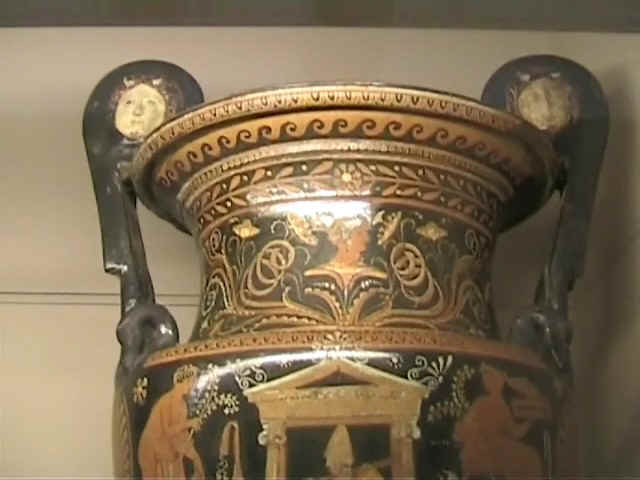
\includegraphics[width=0.5\linewidth]{images/SCP-019.jpg}
    \caption*{SCP-019}
\end{figure}

\bb{项目编号:}SCP-019

\bb{项目等级:}Keter

\bb{特殊收容措施:}SCP-019保存于装有焚化炉的3米X 3米 X 4米的钢筋混凝土房间内的一个炉格上。焚化炉关闭时,房间必须维持在零(0)摄氏度。与该房间一窗之隔的监控室必须时刻保持监视SCP-019的动向,一旦发现SCP-019-2个体出现,须即刻启动焚化炉。万一SCP-019-2发生暴动,可以用普通枪械可以抹杀单独个体,火焰喷射器可以有效地对付大规模爆发。SCP-019本体任何时候都必须直立放置。

\bb{描述:}SCP-019外观为一个巨型瓷器瓶,高度2.4米,瓶口直径1.8米。虽然没有办法确定其确切的出产年代,但从其款式和花纹来看,应该诞生于古希腊时期,SCP-019的表面无法受到任何已知手段的损害。如果以后有任何方法能够成功,SCP-019必须立刻被无条件摧毁。

SCP-019会周期性地产生另一种独立存在的个体。这些个体统称SCP-019-2。它们呈现多种形态,但外观趋向于小体型人形(可能具有动物特征),并且都怀有高度敌意。它们会用牙齿和爪子进行攻击。虽然极度脆弱(而且极度易燃),但是当数量够多时,它们仍可能构成严重威胁。

\begin{figure}[H]
    \centering
    
\includegraphics[width=0.5\linewidth]{images/SCP-019-2.jpg}
    \caption*{SCP-019-2个体}
\end{figure}

当保存于零(0)摄氏度时且处于静止状态时,SCP-019-2个体以每小时一(1)个的频率从SCP-019出现。已知下列条件会影响SCP-019-2的出现速率:

\begin{itemize}
\item 移动SCP-019
\item SCP-019本体受到威胁
\item 极端的高低温
\item 周围环境突然改变
\item 往SCP-019内放入任何物体包括无机物和有机物(将会引发大量个体产生的“潮水”效应)
\end{itemize}

以下条件存在影响SCP-019-2的出现速率的可能性

\begin{itemize}
\item SCP-019附近出现人类
\item 当前天气状况
\item 某些特定人物接近SCP-019(有些人比其他人更容易导致SCP-019-2个体加速出现)
\end{itemize}

此外,翻倒或倾斜SCP-019会制造一种反应,使它看起来就像先前就已经“装满”了SCP-019-2个体似般,尽管从上方看进SCP-019里只会注意到一个漆黑的洞口。基于SCP-019-2在项目被干扰时的出现速率,难以对内部腔体进行测量,但怀疑会和在外部测量的结果不一致。

\bb{附录:}SCP-019-2-A档案\\
SCP-019-2的笔录,由Light博士和Vaux博士负责维护。

██\slash ██\slash ████                      \\
SCP-019-2样本从收容室中转移,保存于强固围栏中,并提供水和活鸡作为其食物。样本连续不断地发出微弱而混乱的声音,音调与古希腊语相似。虽然不清楚为什么会如此,但样本并没有展现出比动物更高的智能。

样本存活时间小于48小时,解剖显示对象的骨骼具有普通生物学中稳定的蜂巢结构水平,但骨骼肌极不稳定。其他值得注意的反常之处包括不稳定的呼吸系统,无消化道,实际上也没有其它内部器官。所有其他被捕获的样本都有相似的特征,行为习惯和死亡时间。

笔记:看来它们离开SCP-019后能生存多长时间对他们来说没有意义。 -Vaux博士

██\slash ██\slash ████\\
收容单元因长期受到SCP-019-2个体攻击而遭到轻微损害,原因為新产生的SCP-019-2个体部分身体透明,没有被观测小组监视到。未观察到以前的SCP-019-2具有该特征。监视组会继续追踪并报告更多异常现象

██\slash ██\slash ████\\
监视组报告:部分SCP-019-2个体对焚烧展现出比其它同类更高的抗性。暂假定该特性为SCP-019的防御机制的部分体现。

██\slash ██\slash ████\\
大多数SCP-019-2个体现在几乎完全具备抵御焚化炉的能力。考虑使用酸液池代替焚化炉。对SCP-019-2“进化”的研究正在进行中,并可作为SCP-019-2具有感知能力的证据。
